%%%%%%%%%%%%%%%%%%%%%%%%%%%%%%%%%%%%%%%%%
% Lachaise Assignment
% LaTeX Template
% Version 1.0 (26/6/2018)
%
% This template originates from:
% http://www.LaTeXTemplates.com
%
% Authors:
% Marion Lachaise & François Févotte
% Vel (vel@LaTeXTemplates.com)
%
% License:
% CC BY-NC-SA 3.0 (http://creativecommons.org/licenses/by-nc-sa/3.0/)
% 
%%%%%%%%%%%%%%%%%%%%%%%%%%%%%%%%%%%%%%%%%

%----------------------------------------------------------------------------------------
%	PACKAGES AND OTHER DOCUMENT CONFIGURATIONS
%----------------------------------------------------------------------------------------

\documentclass{article}
% \usepackage[brazil]{babel}
\usepackage{graphicx}
\graphicspath{ {./images/} }

%%%%%%%%%%%%%%%%%%%%%%%%%%%%%%%%%%%%%%%%%
% Lachaise Assignment
% Structure Specification File
% Version 1.0 (26/6/2018)
%
% This template originates from:
% http://www.LaTeXTemplates.com
%
% Authors:
% Marion Lachaise & François Févotte
% Vel (vel@LaTeXTemplates.com)
%
% License:
% CC BY-NC-SA 3.0 (http://creativecommons.org/licenses/by-nc-sa/3.0/)
% 
%%%%%%%%%%%%%%%%%%%%%%%%%%%%%%%%%%%%%%%%%

%----------------------------------------------------------------------------------------
%	PACKAGES AND OTHER DOCUMENT CONFIGURATIONS
%----------------------------------------------------------------------------------------

\usepackage{amsmath,amsfonts,stmaryrd,amssymb} % Math packages

\usepackage{enumerate} % Custom item numbers for enumerations

\usepackage[ruled]{algorithm2e} % Algorithms

\usepackage[framemethod=tikz]{mdframed} % Allows defining custom boxed/framed environments

\usepackage{listings} % File listings, with syntax highlighting
\lstset{
	basicstyle=\ttfamily, % Typeset listings in monospace font
}

\usepackage{derivative} % support for derivatives
\usepackage{siunitx} % support for SI units

\usepackage{empheq} 
\usepackage{xcolor}
\definecolor{lightgreen}{HTML}{90EE90}

%----------------------------------------------------------------------------------------
%	DOCUMENT MARGINS
%----------------------------------------------------------------------------------------

\usepackage{geometry} % Required for adjusting page dimensions and margins

\geometry{
	paper=a4paper, % Paper size, change to letterpaper for US letter size
	top=2.5cm, % Top margin
	bottom=3cm, % Bottom margin
	left=2.5cm, % Left margin
	right=2.5cm, % Right margin
	headheight=14pt, % Header height
	footskip=1.5cm, % Space from the bottom margin to the baseline of the footer
	headsep=1.2cm, % Space from the top margin to the baseline of the header
	%showframe, % Uncomment to show how the type block is set on the page
}

%----------------------------------------------------------------------------------------
%	FONTS
%----------------------------------------------------------------------------------------

\usepackage[utf8]{inputenc} % Required for inputting international characters
\usepackage[T1]{fontenc} % Output font encoding for international characters

\usepackage{XCharter} % Use the XCharter fonts

%----------------------------------------------------------------------------------------
%	COMMAND LINE ENVIRONMENT
%----------------------------------------------------------------------------------------

% Usage:
% \begin{commandline}
%	\begin{verbatim}
%		$ ls
%		
%		Applications	Desktop	...
%	\end{verbatim}
% \end{commandline}

\mdfdefinestyle{commandline}{
	leftmargin=10pt,
	rightmargin=10pt,
	innerleftmargin=15pt,
	middlelinecolor=black!50!white,
	middlelinewidth=2pt,
	frametitlerule=false,
	backgroundcolor=black!5!white,
	frametitle={Command Line},
	frametitlefont={\normalfont\sffamily\color{white}\hspace{-1em}},
	frametitlebackgroundcolor=black!50!white,
	nobreak,
}

% Define a custom environment for command-line snapshots
\newenvironment{commandline}{
	\medskip
	\begin{mdframed}[style=commandline]
}{
	\end{mdframed}
	\medskip
}

%----------------------------------------------------------------------------------------
%	FILE CONTENTS ENVIRONMENT
%----------------------------------------------------------------------------------------

% Usage:
% \begin{file}[optional filename, defaults to "File"]
%	File contents, for example, with a listings environment
% \end{file}

\mdfdefinestyle{file}{
	innertopmargin=1.6\baselineskip,
	innerbottommargin=0.8\baselineskip,
	topline=false, bottomline=false,
	leftline=false, rightline=false,
	leftmargin=2cm,
	rightmargin=2cm,
	singleextra={%
		\draw[fill=black!10!white](P)++(0,-1.2em)rectangle(P-|O);
		\node[anchor=north west]
		at(P-|O){\ttfamily\mdfilename};
		%
		\def\l{3em}
		\draw(O-|P)++(-\l,0)--++(\l,\l)--(P)--(P-|O)--(O)--cycle;
		\draw(O-|P)++(-\l,0)--++(0,\l)--++(\l,0);
	},
	nobreak,
}

% Define a custom environment for file contents
\newenvironment{file}[1][File]{ % Set the default filename to "File"
	\medskip
	\newcommand{\mdfilename}{#1}
	\begin{mdframed}[style=file]
}{
	\end{mdframed}
	\medskip
}

%----------------------------------------------------------------------------------------
%	NUMBERED QUESTIONS ENVIRONMENT
%----------------------------------------------------------------------------------------

% Usage:
% \begin{question}[optional title]
%	Question contents
% \end{question}

\mdfdefinestyle{question}{
	innertopmargin=1.2\baselineskip,
	innerbottommargin=0.8\baselineskip,
	roundcorner=5pt,
	nobreak,
	singleextra={%
		\draw(P-|O)node[xshift=1em,anchor=west,fill=white,draw,rounded corners=5pt]{%
		Question \theQuestion\questionTitle};
	},
}

\newcounter{Question} % Stores the current question number that gets iterated with each new question

% Define a custom environment for numbered questions
\newenvironment{question}[1][\unskip]{
	\bigskip
	\stepcounter{Question}
	\newcommand{\questionTitle}{~#1}
	\begin{mdframed}[style=question]
}{
	\end{mdframed}
	\medskip
}

%----------------------------------------------------------------------------------------
%	WARNING TEXT ENVIRONMENT
%----------------------------------------------------------------------------------------

% Usage:
% \begin{warn}[optional title, defaults to "Warning:"]
%	Contents
% \end{warn}

\mdfdefinestyle{warning}{
	topline=false, bottomline=false,
	leftline=false, rightline=false,
	nobreak,
	singleextra={%
		\draw(P-|O)++(-0.5em,0)node(tmp1){};
		\draw(P-|O)++(0.5em,0)node(tmp2){};
		\fill[black,rotate around={45:(P-|O)}](tmp1)rectangle(tmp2);
		\node at(P-|O){\color{white}\scriptsize\bf !};
		\draw[very thick](P-|O)++(0,-1em)--(O);%--(O-|P);
	}
}

% Define a custom environment for warning text
\newenvironment{warn}[1][Warning:]{ % Set the default warning to "Warning:"
	\medskip
	\begin{mdframed}[style=warning]
		\noindent{\textbf{#1}}
}{
	\end{mdframed}
}

%----------------------------------------------------------------------------------------
%	INFORMATION ENVIRONMENT
%----------------------------------------------------------------------------------------

% Usage:
% \begin{info}[optional title, defaults to "Info:"]
% 	contents
% 	\end{info}

\mdfdefinestyle{info}{%
	topline=false, bottomline=false,
	leftline=false, rightline=false,
	nobreak,
	singleextra={%
		\fill[black](P-|O)circle[radius=0.4em];
		\node at(P-|O){\color{white}\scriptsize\bf i};
		\draw[very thick](P-|O)++(0,-0.8em)--(O);%--(O-|P);
	}
}

% Define a custom environment for information
\newenvironment{info}[1][Info:]{ % Set the default title to "Info:"
	\medskip
	\begin{mdframed}[style=info]
		\noindent{\textbf{#1}}
}{
	\end{mdframed}
}

%----------------------------------------------------------------------------------------
%	EQUATION BOXES
%----------------------------------------------------------------------------------------
 % Include the file specifying the document structure and custom commands

%----------------------------------------------------------------------------------------
%	ASSIGNMENT INFORMATION
%----------------------------------------------------------------------------------------

\title{Critical Systems Evaluation} % Title of the assignment

\author{First Homework List\\ Equipe: \texttt{aasb2, acn2, pvoa, vbmp}} % Author name and email address

\date{CIn, UFPE --- \today} % University, school and/or department name(s) and a date

%----------------------------------------------------------------------------------------

\begin{document}

\maketitle % Print the title

%----------------------------------------------------------------------------------------
%	PROBLEM 1
%----------------------------------------------------------------------------------------
\begin{question}
    Comment your understanding of:
    \begin{enumerate}[label=(\alph*)]
        \item grouped and ungrouped data set
        \item complete and censored data
        \item  operational data and test generated data
        \item left-censoring
        \item right-censoring type 1 and type 2
        \item and multi censored data
    \end{enumerate}
    \end{question}

\begin{enumerate}[label=(\alph*)]
    \item \textbf{grouped and ungrouped data set:} 
    
        Grouped data set is organized into intervals or groups, and you're given the frequency of observations within each group. On ungrouped data set each individual observation is listed separately without grouping into intervals.
           
    \item \textbf{complete and censored data:}
    
        Complete data is a dataset where every data point has been observed or measured without any missing values.
        Censored data, is data in which the information about some values is incomplete because the measurements are constrained in some way. This can be left-censored, right-censored, or interval-censored.
        
    \item \textbf{operational data and test generated data:}
    
        Operational Data, the is data collected during the normal operation of a system or process.
        Test-Generated Data, the data specifically created for testing purposes, often in a controlled environment to assess the performance of a system or model.
    \item \textbf{left-censoring:}
    
        Occurs when the lower bound of a measurement is known, but values below this bound are not observed or recorded. It's a form of incomplete data where the true values are censored on the left side.
        
    \item \textbf{light-censoring type 1 and type 2:}
    
       In the right-censoring type 1 the values above a certain threshold are not observed. The data is truncated at the right end.
       In the right-censoring type 2 the values above a certain threshold are recorded as being above that threshold, but the exact values are not known. This is common in survival analysis, where the event of interest may not have occurred for some subjects.
        
    \item \textbf{and multi censored data:}
    
        Refers to a situation where data is censored in multiple ways. For example, you might have both left-censored and right-censored data in a single dataset.
\end{enumerate}

%----------------------------------------------------------------------------------------
%	PROBLEM 3
%----------------------------------------------------------------------------------------

\setcounter{Question}{2}
\begin{question}
Assume a set of sixty servers ($n = 60$) were place in an accelerate reliability test. The test finished when all servers
presented a failure. In Table 1, Columns TTF$i$ present the time to failure of the servers in ascending order.
\ref{table:4} (complete data).
    \begin{enumerate}[label=(\alph*)]
        \item Using a non-parametric method, calculate $R^(t)$, and $F^(t)$ at $t = 1800.82h$
        \item  Draw $R^(t) \times t$, and $F^(t) \times t$
        \item  Calculate $MTTF$
        \item Estimate the confidence interval of the $MTTF$ using non-parametric bootstrap.
    \end{enumerate}
    
\end{question}

\begin{table}[H]
    \centering
    \begin{tabular}{|*{12}{c|}}
        \hline
        $i$ & $TTFi$ (h) & $TTFi$ & $TTFi$ (h) & $TTFi$ & $TTFi$ (h) & $TTFi$ \\
        \hline
        1 & 1088.55 & 1808.22 & 2295.93 & 2677.00 & 3715.81 & 4262.82 \\
        2 & 1421.70 & 1808.77 & 2368.95 & 2734.39 & 3716.82 & 4362.63 \\
        3 & 1501.50 & 1835.81 & 2438.96 & 2795.40 & 3770.61 & 4500.37 \\
        4 & 1534.56 & 1859.16 & 2509.08 & 2968.35 & 3808.22 & 4658.01 \\
        5 & 1611.89 & 1889.69 & 2592.39 & 3106.45 & 3823.24 & 4775.04 \\
        6 & 1629.61 & 2044.81 & 2601.27 & 3282.68 & 3844.85 & 4798.53 \\
        7 & 1665.32 & 2065.61 & 2629.69 & 3601.69 & 3943.01 & 4958.32 \\
        8 & 1740.20 & 2179.10 & 2635.79 & 3623.20 & 3988.39 & 5260.35 \\
        9 & 1799.39 & 2249.68 & 2660.02 & 3627.13 & 4118.64 & 5508.57 \\
        10 & 1800.82 & 2261.86 & 2674.43 & 3631.10 & 4216.89 & 6968.88 \\
        j & 1 & 2 & 3 & 4 & 5 & 6 \\
        \hline
    \end{tabular}
    \caption{Your Table Caption Here}
    \label{table:4}
\end{table}
\begin{enumerate}[label=(\alph*)]
    \item Using a non-parametric method, calculate $R^(t)$, and $F^(t)$ at $t = 1800.82h$       \begin{flushleft}
            The first step is to have the table in ascending order, which in this case, has already been provided to us with such an order

            Now we have to determine the number of servers that failed before or at $t = 1800.82$ hours, which can be calculated as

            \(R^(t) = \frac{\text{Numbers of servers surviving at t}}{\text{Total number of servers}}\)

            and 
            
            \(F^(t) = 1 - R^(t)\)

            With the info of the table we know that the number of servers failing before or at t = 1800.82 hours is 10, and the total is 60.

            \(R^(1800.82) = \frac{10}{60}\)  \\

            \(F^(1800.82) = 1 - \frac{10}{60}\) \\

        
            So, the non-parametric estimates $R^(1800.82)$ and $F^(1800.82)$ are approximately:
            \[\fbox{$\hat{R}(1800.82) = 0.1666$}\]
            \[\fbox{$\hat{F}(1800.82) = 0.8333$}\]

        \end{flushleft}

    \item Draw $R^(t) \times t$, and $F^(t) \times t$
        \begin{flushleft}
            \begin{figure}[H]
                \centering
                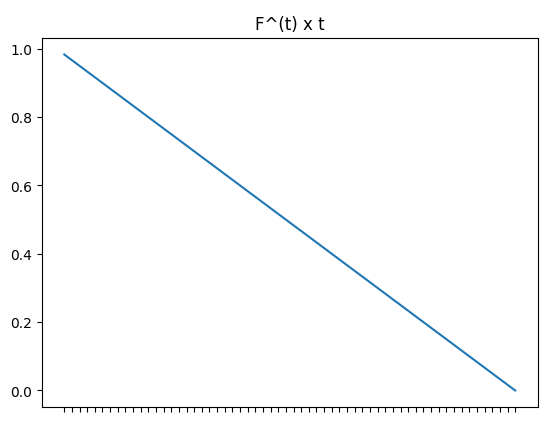
\includegraphics[width=0.7\linewidth]{ft_q3.png}
                \label{fig:F^(t) x t}
            \end{figure}
        \end{flushleft}

        \begin{flushleft}
            \begin{figure}[H]
                \centering
                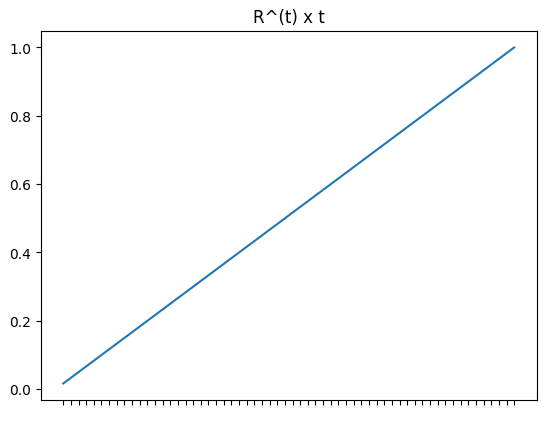
\includegraphics[width=0.7\linewidth]{rt_q3.png}
                \label{fig:R^(t) x t}
            \end{figure}
        \end{flushleft}
    

    \item Calculate $MTTF$
        The Mean Time To Failure ($MTTF$) can be calculated by finding the average time to failure for all the servers. The formula for $MTTF$ is:
        \begin{gather*}
            MTTF = \frac{\text{Sum of TTF for all units}}{\text{Number of units}} \\
            MTTF = \frac{1088.55+1808.22+\cdots+6968.88}{60} \\
            MTTF = \frac{1088.55+1808.22+\cdots+6968.88}{60} \\
            MTTF = \frac{182.250,15}{60} \\
            \fbox{MTTF = 3037.50}
        \end{gather*}

        
    \item Estimate the confidence interval of the $MTTF$ using non-parametric bootstrap.
        \begin{flushleft}
                \item Using the following code in python to apply the non-parametric bootstrap to the data:

            \lstset{
              basicstyle=\ttfamily,
              numbers=left,
              numberstyle=\tiny\color{gray},
              breaklines=true,
              keywordstyle=\color{blue},
              commentstyle=\color{green!40!black},
              stringstyle=\color{orange},
              frame=single,
              language=Python
            }
        
        
            \begin{lstlisting}
            import numpy as np
            
            # Given data
            failure_times = np.array([
                1088.55, 1808.22, 2295.93, 2677.00, 3715.81, 4262.82,
                1421.70, 1808.77, 2368.95, 2734.39, 3716.82, 4362.63,
                1501.50, 1835.81, 2438.96, 2795.40, 3770.61, 4500.37,
                1534.56, 1859.16, 2509.08, 2968.35, 3808.22, 4658.01,
                1611.89, 1889.69, 2592.39, 3106.45, 3823.24, 4775.04,
                1629.61, 2044.81, 2601.27, 3282.68, 3844.85, 4798.53,
                1665.32, 2065.61, 2629.69, 3601.69, 3943.01, 4958.32,
                1740.20, 2179.10, 2635.79, 3623.20, 3988.39, 5260.35,
                1799.39, 2249.68, 2660.02, 3627.13, 4118.64, 5508.57,
                1800.82, 2261.86, 2674.43, 3631.10, 4216.89, 6968.88
            ])
            
            # Number of bootstrap samples
            num_samples = 1000
            
            # Initialize an array to store bootstrap MTTF values
            bootstrap_mttf = np.zeros(num_samples)
            
            # Bootstrap resampling and MTTF calculation
            for i in range(num_samples):
                bootstrap_sample = np.random.choice(failure_times, size=len(failure_times), replace=True)
                bootstrap_mttf[i] = np.mean(bootstrap_sample)
            
            # Calculate the confidence interval
            confidence_interval = np.percentile(bootstrap_mttf, [2.5, 97.5])
            
            print("Bootstrap Mean Time To Failure (MTTF):", np.mean(bootstrap_mttf))
            print("Bootstrap 95% Confidence Interval:", confidence_interval)
            \end{lstlisting}
            
            
            Bootstrap Mean Time To Failure (MTTF): $3031.8683h$ \\
            \fbox{Bootstrap 95\% Confidence Interval: $[2711.7305h,~ 3336.1719h]$}
        \end{flushleft}

%----------------------------------------------------------------------------------------
%	PROBLEM 4
%----------------------------------------------------------------------------------------
\begin{question}
Sixty servers ($n = 60$) went through an accelerated reliability test. However, not all servers were kept until the end of the test; that is, some of them were removed (censured) from the test when they were still
operational. Table 2 is a multi-column table, where (j,i), j $\in$ {1,2,3}, and i $\in$ {1..20}. The 
table shows the event times (Columns $ti$) - failure or censoring. Columns $\delta i$ represent failures (1) or censoring (0). Columns $ti$ - $ti-1$ present the time interval between two consecutive events, and Columns i specify the event order.
\ref{table:4} (complete data).
    \begin{enumerate}[label=(\alph*)]
        \item Using a non-parametric method draw the graphs a) $R^(t) \times t$ and $F^(t) \times t$
        \item Estimate $R^(3088.73h)$
    \end{enumerate}
\end{question}
\begin{enumerate}[label=(\alph*)]
    \item Using a non-parametric method draw the graphs a) $R^(t) \times t$ and $F^(t) \times t$
    \begin{flushleft}
            \item Using the following code in python to apply the non-parametric bootstrap to the data:

            \lstset{
              basicstyle=\ttfamily,
              numbers=left,
              numberstyle=\tiny\color{gray},
              breaklines=true,
              keywordstyle=\color{blue},
              commentstyle=\color{green!40!black},
              stringstyle=\color{orange},
              frame=single,
              language=Python
            }
        
        
            \begin{lstlisting}
            # Given data
            t_values = np.array([
                19.11, 1544.00, 4196.34,
                25.62, 1558.04, 4278.78,
                269.48, 1947.92, 4623.43,
                431.81, 2115.51, 4668.51,
                520.48, 2307.92, 4862.93,
                533.40, 2347.95, 5120.96,
                684.16, 2413.24, 5400.25,
                709.78, 2509.03, 5693.01,
                830.20, 2782.08, 6120.47,
                861.62, 3088.73, 6656.40,
                897.72, 3153.86, 8042.32,
                915.40, 3156.66, 8893.73,
                939.79, 3162.79, 9022.43,
                1037.99, 3276.37, 9216.15,
                1113.06, 3313.52, 9301.77,
                1276.45, 3323.28, 9379.77,
                1283.82, 3492.84, 9681.48,
                1353.88, 3559.71, 10351.36,
                1425.11, 3966.95, 10993.42,
                1489.69, 3978.91, 13496.11
            ])
            
            delta_values = np.array([
                0, 1, 0, 1, 0,
                1, 1, 1, 1, 1,
                1, 0, 1, 1, 1,
                1, 0, 1, 0, 1,
                0, 1, 0, 1, 0,
                1, 0, 1, 0, 1,
                1, 0, 1, 0, 1,
                0, 1, 0, 1, 0,
                1, 0, 1, 1, 1,
                0, 1, 1, 1, 1,
                1, 1, 0, 1, 1,
                1, 0, 1, 1, 1,
                0, 0, 1, 0, 1,
                0, 1, 1, 1, 0,
                0, 1, 0, 1, 0,
                1, 0, 1, 1, 0
            ])
            
            delta_values = np.array([0, 1, 0, 1, 1, 1, 1, 0, 1, 1, 1, 0, 0, 1, 0, 1, 0, 1, 1, 0, 1, 0, 1, 0, 1, 1, 1, 0, 1, 1, 1, 1, 1, 1, 0, 1, 0, 1, 1, 0, 0, 0, 0, 1, 1, 1, 1, 1, 1, 1, 1, 1, 1, 1, 0, 0, 1, 1, 0, 0]) 
            
            # Create Kaplan-Meier estimator
            kmf = KaplanMeierFitter()
            print(len(t_values))
            kmf.fit(durations=t_values, event_observed=delta_values)
            
            # Plotting R(t)
            plt.figure(figsize=(12, 6))
            kmf.plot_survival_function(ci_show=False)
            plt.title('Reliability Estimate $\\hat{R}(t)$')
            plt.xlabel('Time (hours)')
            plt.ylabel('Reliability')
            
            # Plotting F(t)
            plt.figure(figsize=(12, 6))
            kmf.plot_cumulative_density(ci_show=False)
            plt.title('Cumulative Distribution Function $\\hat{F}(t)$')
            plt.xlabel('Time (hours)')
            plt.ylabel('Cumulative Probability')
            
            plt.show()
            \end{lstlisting}

        \begin{flushleft}
            \begin{figure}[H]
                \centering
                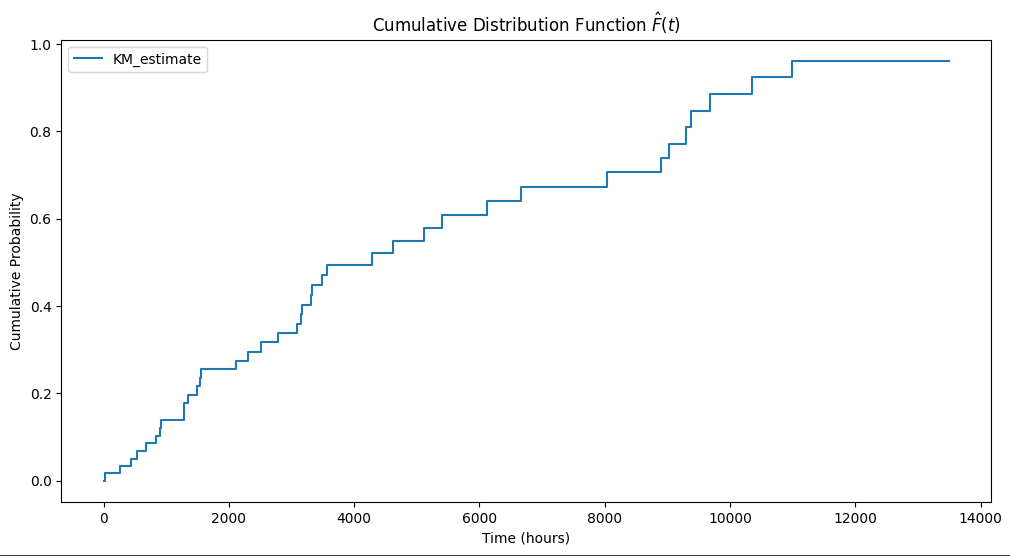
\includegraphics[width=0.7\linewidth]{ft_q4.png}
                \label{fig:q4Ftt}
            \end{figure}
        \end{flushleft}

        \begin{flushleft}
            \begin{figure}[H]
                \centering
                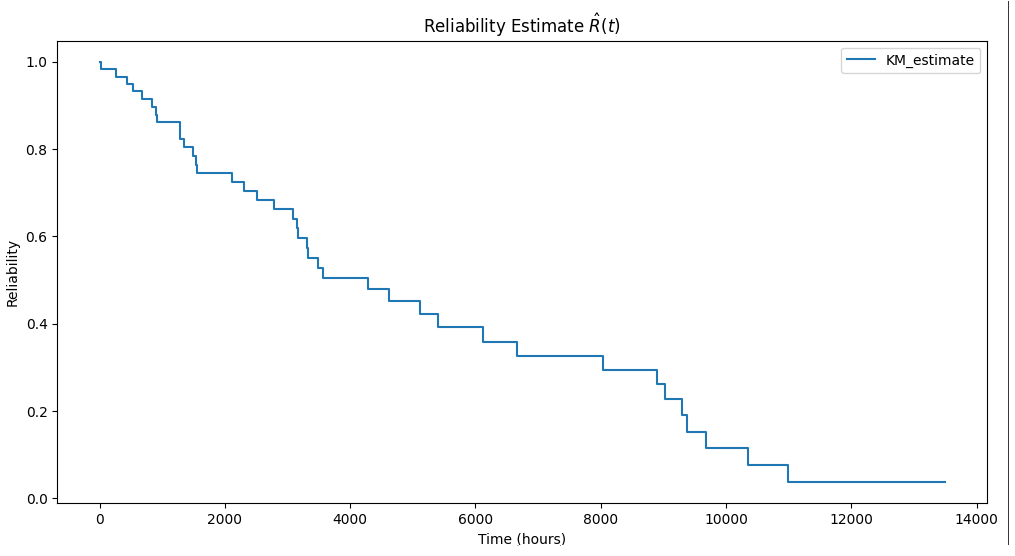
\includegraphics[width=0.7\linewidth]{rt_q4.png}
                \label{fig:q4Rtt}
            \end{figure}
        \end{flushleft}

        \end{flushleft}
        
    \item Estimate $R^(8500h)$ 
        We are going to use the cumulative number of failures and the cumulative number of censored observations, which are given, respectively, by:
        
        \(\text{Cumulative number of failures} = \sum_{n}^{n} \delta i)\) \\

        \(\text{Number of censored observations} = \sum_{n}^{ti}(1 - \delta i)\) \\
        
        \(R^(t) = exp(-\frac{\sum_{n}^{ti} \delta i}{n})\) \\
        
        where $n$ is the total number of servers.
    \begin{flushleft}
            \item Using the following code in python to apply the non-parametric bootstrap to the data:

            \lstset{
              basicstyle=\ttfamily,
              numbers=left,
              numberstyle=\tiny\color{gray},
              breaklines=true,
              keywordstyle=\color{blue},
              commentstyle=\color{green!40!black},
              stringstyle=\color{orange},
              frame=single,
              language=Python
            }
        
            \begin{lstlisting}
            # import numpy as np
            
            # # Given data
            # failure_times = np.array([
            #     1088.55, 1808.22, 2295.93, 2677.00, 3715.81, 4262.82,
            #     1421.70, 1808.77, 2368.95, 2734.39, 3716.82, 4362.63,
            #     1501.50, 1835.81, 2438.96, 2795.40, 3770.61, 4500.37,
            #     1534.56, 1859.16, 2509.08, 2968.35, 3808.22, 4658.01,
            #     1611.89, 1889.69, 2592.39, 3106.45, 3823.24, 4775.04,
            #     1629.61, 2044.81, 2601.27, 3282.68, 3844.85, 4798.53,
            #     1665.32, 2065.61, 2629.69, 3601.69, 3943.01, 4958.32,
            #     1740.20, 2179.10, 2635.79, 3623.20, 3988.39, 5260.35,
            #     1799.39, 2249.68, 2660.02, 3627.13, 4118.64, 5508.57,
            #     1800.82, 2261.86, 2674.43, 3631.10, 4216.89, 6968.88
            # ])
            
            # # Number of bootstrap samples
            # num_samples = 1000
            
            # # Initialize an array to store bootstrap MTTF values
            # bootstrap_mttf = np.zeros(num_samples)
            
            # # Bootstrap resampling and MTTF calculation
            # for i in range(num_samples):
            #     bootstrap_sample = np.random.choice(failure_times, size=len(failure_times), replace=True)
            #     bootstrap_mttf[i] = np.mean(bootstrap_sample)
            
            # # Calculate the confidence interval
            # confidence_interval = np.percentile(bootstrap_mttf, [2.5, 97.5])
            
            # print("Bootstrap Mean Time To Failure (MTTF):", np.mean(bootstrap_mttf))
            # print("Bootstrap 95% Confidence Interval:", confidence_interval)
            
            import numpy as np
            
            # Given data
            t_values = np.array([
                19.11, 1544.00, 54.31, 4196.34, 217.43,
                25.62, 1558.04, 1503.73, 4278.78, 4061.36,
                269.48, 1947.92, 444.19, 4623.43, 562.08,
                431.81, 2115.51, 1671.32, 4668.51, 4106.43,
                520.48, 2307.92, 636.60, 4862.93, 756.50,
                533.40, 2347.95, 1711.35, 5120.96, 4364.45,
                684.16, 2413.24, 701.89, 5400.25, 1035.79,
                709.78, 2509.03, 1807.15, 5693.01, 4657.22,
                830.20, 2782.08, 974.93, 6120.47, 1463.25,
                861.62, 3088.73, 2113.80, 6656.40, 5193.15,
                897.72, 3153.86, 1040.06, 8042.32, 2849.17,
                915.40, 3156.66, 2116.60, 8893.73, 6044.55,
                939.79, 3162.79, 1046.19, 9022.43, 2977.88,
                1037.99, 3276.37, 2230.17, 9216.15, 6238.27,
                1113.06, 3313.52, 1083.35, 9301.77, 3063.49,
                1276.45, 3323.28, 2239.93, 9379.77, 6316.28,
                1283.82, 3492.84, 1252.91, 9681.48, 3365.21,
                1353.88, 3559.71, 2306.80, 10351.36, 6986.15,
                1425.11, 3966.95, 1660.15, 10993.42, 4007.27,
                1489.69, 3978.91, 2318.77, 13496.11, 9488.83
            ])
            
            delta_values = np.array([
                0, 1, 0, 1, 0,
                1, 1, 1, 1, 1,
                1, 0, 1, 1, 1,
                1, 0, 1, 0, 1,
                0, 1, 0, 1, 0,
                1, 0, 1, 0, 1,
                1, 0, 1, 0, 1,
                0, 1, 0, 1, 0,
                1, 0, 1, 1, 1,
                0, 1, 1, 1, 1,
                1, 1, 0, 1, 1,
                1, 0, 1, 1, 1,
                0, 0, 1, 0, 1,
                0, 1, 1, 1, 0,
                0, 1, 0, 1, 0,
                1, 0, 1, 1, 0
            ])
            
            # Identify events up to t = 8500 hours
            events_8500 = t_values[t_values <= 8500]
            delta_8500 = delta_values[:len(events_8500)]
            
            # Calculate cumulative sums
            cumulative_failures = np.sum(delta_8500)
            cumulative_censored = np.sum(1 - delta_8500)
            
            # Estimate R(t) at t = 8500 hours
            n_servers = 60
            R_8500 = np.exp(-cumulative_failures / n_servers)
            
            print(f"Estimated R(8500h): {R_8500:.4f}")
            \end{lstlisting}
        Which gives us the result of:
        
        \fbox{$\hat{R}(8500h): 0.4346$}
        \end{flushleft}
        
\end{enumerate}

\end{enumerate}

%----------------------------------------------------------------------------------------
%	PROBLEM 5
%----------------------------------------------------------------------------------------
\setcounter{Question}{4}
\begin{question}
    Table 3 summarizes the reliability data test of eighty servers $(n = 80)$ during $13500h$. Inspections were carried out every week $(500h)$. The whole observation was finished at $13500h$. Table 3 shows the time instants that represent the end of each of the twenty-seven intervals $(Column \ t_i)$, the number of failed servers in the respective interval $(Column \ r_i)$, and the number of censored computer in the interval $(Column \ c_i)$. Adopted a non-parametric method to draw the graphs
    \begin{enumerate}[label=(\alph*)]
        \item $\hat{R}(t) \times t$
        \item $\hat{F}(t) \times t$
        \item Estimate $\hat{R}(8500h)$
    \end{enumerate}
\end{question}

\begin{enumerate}[label=(\alph*)]
    \item We'll use the non-parametric Kaplan-Meier estimator to calculate the desired functions. This method is appropriate for this dataset since it can correctly account for right-censored data. For the survival function $R(t)$, we have
    \[\hat{R}(t) = \prod_{i: t_i<t} \left(1- \frac{d_i}{n_i}\right)\]
    Where $d_i$ is the number of failures at time $t_i$, and $n_i$ is the survivors up to time $t_i$. That is, the total number of servers minus the sum of all failures and censored data before $t_i$.
    We used the provided Life Time Data Analysis spreadsheet to compute the results for the Kaplan-Meier estimator.

    \begin{figure}[H]
        \centering
        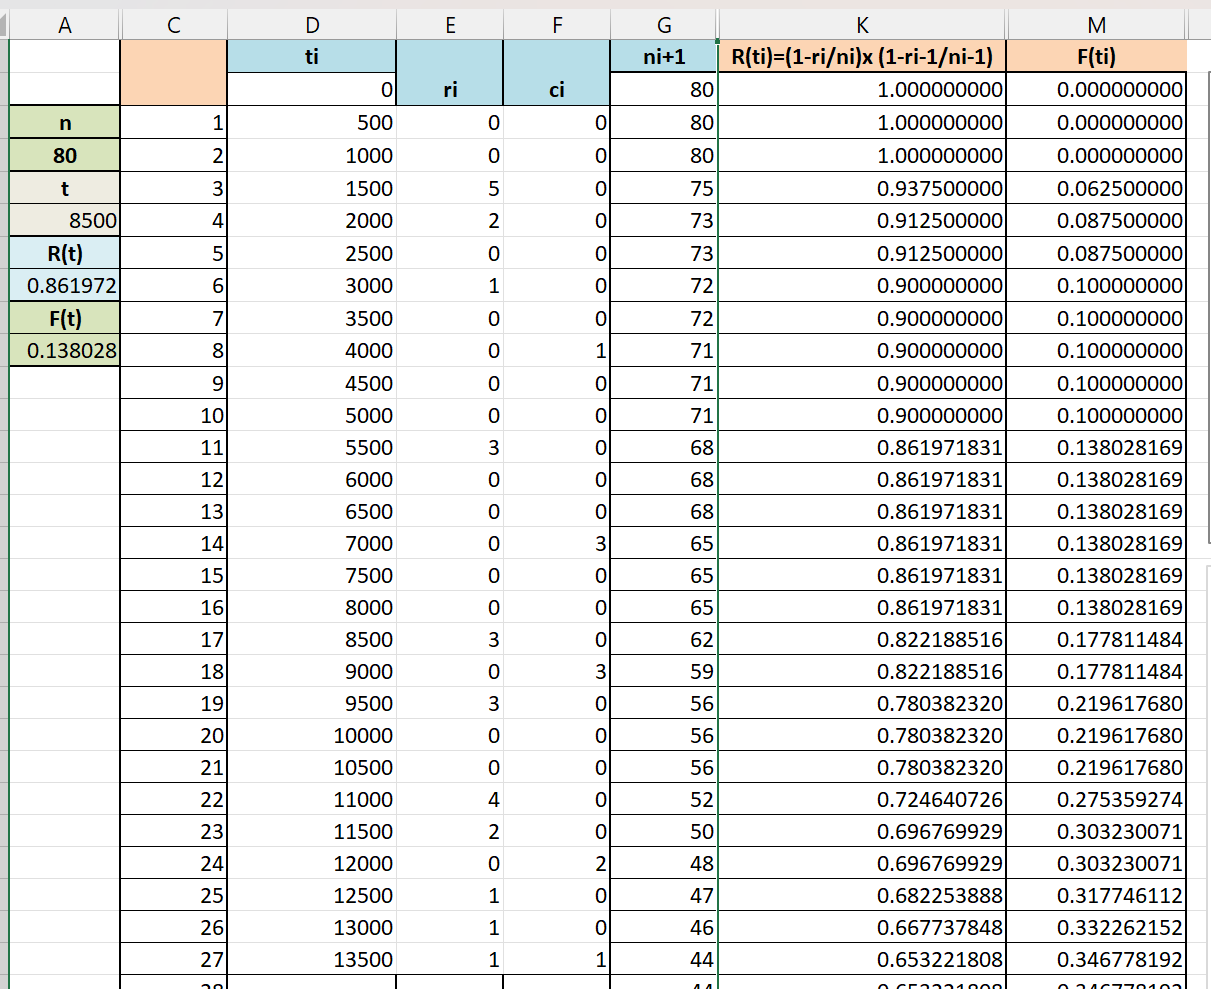
\includegraphics[width=0.5\linewidth]{q3_sheet.png}
        \caption{Kaplan-Meier spreadsheet results}
        \label{fig:q3_km1}
    \end{figure}

    With the resulting values, we can plot the curve for the $\hat{R}(t)$ and $\hat{F}(t)$ functions

    \begin{figure}[H]
        \centering
        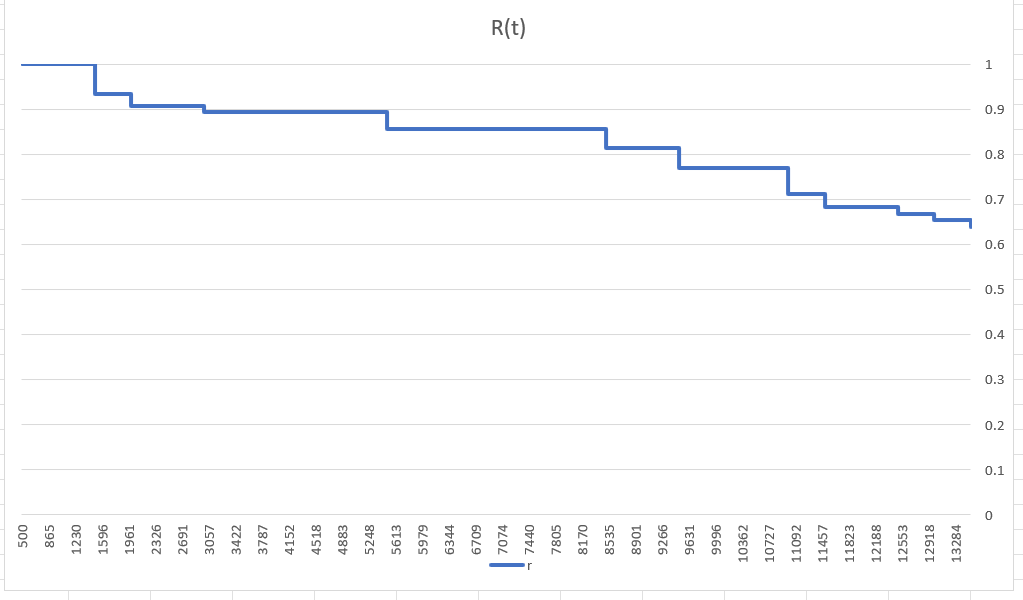
\includegraphics[width=0.8\linewidth]{q3_rt.png}
        \caption{$\hat{R}(t) \times t$}
        \label{fig:q3_km_rt}
    \end{figure}

    We can see that the reliability is fairly stable, being above 0.65 after 13500h
    \item We know that $\hat{F}(t) = 1 - \hat{R}(t)$, so we can take the complement of the values from $\hat{R}(t)$ to plot $\hat{F}(t)$

    \begin{figure}[H]
        \centering
        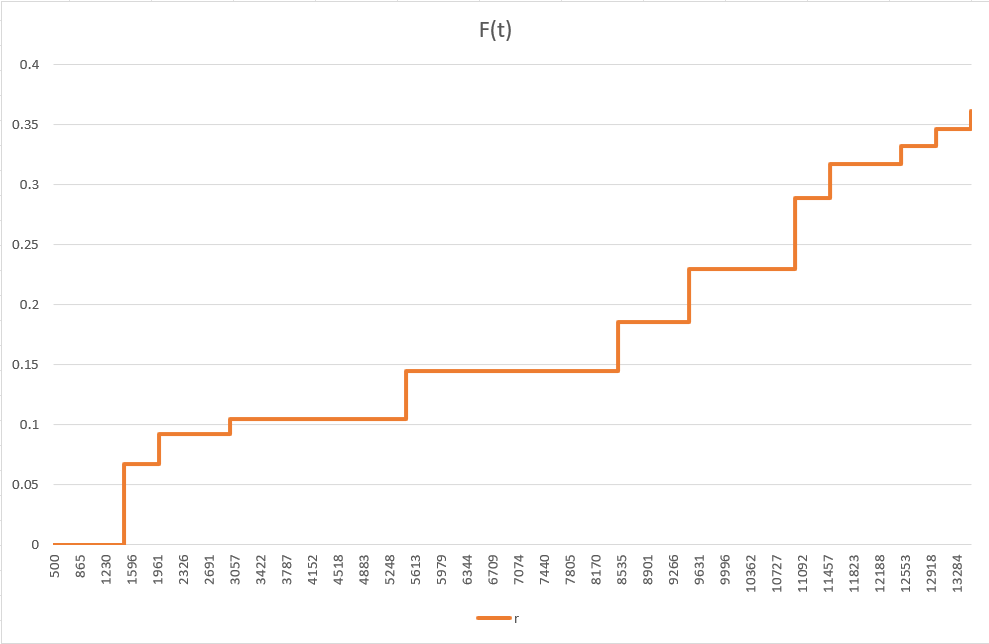
\includegraphics[width=0.8\linewidth]{q3_ft.png}
        \caption{$\hat{F}(t) \times t$}
        \label{fig:q3_km_ft}
    \end{figure}

    \item As $t=8500$ is actually one of our data points, we can use the value we estimated for $t=8500$ directly for our reliability estimate, thus, \fbox{$\hat{R}(8500) \approx 0.822$}. Alternatively, we can run a regression on our data points, and estimate the reliability at that point using that regression. In case of a linear regression, we get $\hat{R}(8500) \approx 0.861$.
\end{enumerate}

%----------------------------------------------------------------------------------------
%	PROBLEM 7
%----------------------------------------------------------------------------------------

\setcounter{Question}{6}
\begin{question}
    What are the pros and cons of the following parametric reliability data analysis:
    \begin{enumerate}[label=(\alph*)]
        \item graphical methods

        \item methods of moments, and
        \item  maximum likelihood estimation methods.
    \end{enumerate}
\end{question}

\begin{enumerate}[label=(\alph*)]
    \item \textbf{Graphical methods:}

          Pros:
          \begin{itemize}
              \item Easy and simple to use
              \item Can be visually checked
          \end{itemize}
          Cons:
          \begin{itemize}
              \item They are not precise
          \end{itemize}

    \item \textbf{Methods of moments:}

          Pros:
          \begin{itemize}
              \item Easy to implement
              \item Flexibility
              \item  Does not depend on distibution assumption
          \end{itemize}
          Cons:
          \begin{itemize}
              \item Sensitive to outliers
              \item Might ignore some distribution aspects
          \end{itemize}

    \item \textbf{Likelihood estimation methods:}

          Pros:
          \begin{itemize}
              \item Less Likely to Be Biased
          \end{itemize}
          Cons:
          \begin{itemize}
              \item Not precise for small number of failures
              \item It might be hard to calculate in some cases
          \end{itemize}
\end{enumerate}

%----------------------------------------------------------------------------------------
%	PROBLEM 8
%----------------------------------------------------------------------------------------

\begin{question}
    Assume the reliability experiment in which sixty servers (n = 60) were observed in an accelerated reliability test. The times each server failed were recorded in Table \ref{table:4} (complete data).
    \begin{enumerate}[label=(\alph*)]
        \item Conduct an exploratory analysis and choose a candidate probability distribution representing the data set.
        \item  Obtain a point estimate of distribution parameters and conduct goodness of fitting. If the candidate distribution does not fit the data set, choose another one until finding a
              suitable distribution.
        \item  Obtain a point estimate of the $MTTF$
        \item Estimate the $MTTF$ confidence interval, adopting 5\% of significance using a semi-parametric bootstrap.
        \item  Estimate the $R(t)$, $F(t)$, $f(t)$ and $\lambda(t)$ at $1000 h$
    \end{enumerate}

\end{question}

\begin{table}[H]
    \centering
    \begin{tabular}{|*{12}{c|}}
        \hline
        $i$ & $t_i$ (h) & $i$ & $t_i$ (h) & $i$ & $t_i$ (h) & $i$ & $t_i$ (h) & $i$ & $t_i$ (h) & $i$ & $t_i$ (h) \\
        \hline
        1   & 765.32    & 11  & 1822.54   & 21  & 515.21    & 31  & 4569.68   & 41  & 408.16    & 51  & 338.18    \\
        2   & 736.36    & 12  & 2026.03   & 22  & 5400.53   & 32  & 4104.01   & 42  & 1509.31   & 52  & 197.89    \\
        3   & 4688.02   & 13  & 211.91    & 23  & 1460.71   & 33  & 728.45    & 43  & 434.26    & 53  & 584.37    \\
        4   & 2181.27   & 14  & 1109.13   & 24  & 1672.60   & 34  & 1188.55   & 44  & 2005.96   & 54  & 86.76     \\
        5   & 4085.90   & 15  & 1189.89   & 25  & 640.21    & 35  & 640.83    & 45  & 924.12    & 55  & 2204.17   \\
        6   & 9044.38   & 16  & 1348.37   & 26  & 711.69    & 36  & 5613.10   & 46  & 1510.17   & 56  & 6591.52   \\
        7   & 3573.45   & 17  & 389.56    & 27  & 190.62    & 37  & 247.44    & 47  & 2548.00   & 57  & 6023.71   \\
        8   & 7201.78   & 18  & 3563.30   & 28  & 4266.00   & 38  & 1647.28   & 48  & 157.32    & 58  & 398.62    \\
        9   & 1237.32   & 19  & 2082.53   & 29  & 1087.26   & 39  & 500.76    & 49  & 399.17    & 59  & 4064.59   \\
        10  & 740.13    & 20  & 3322.64   & 30  & 489.08    & 40  & 3510.87   & 50  & 2020.38   & 60  & 2467.03   \\
        \hline
    \end{tabular}
    \label{table:4}
\end{table}
\begin{enumerate}[label=(\alph*)]
    \item The result of the exploratory analysis was the following:
          \begin{flushleft}
              Sample Size, $n$: 60 \\
              Mean: 2089.64000 \\
              Median: 1404.54000 \\
              Midrange: 4565.57000 \\
              RMS: 2896.88557 \\
              Variance, $s^2$: 4093576.93357 \\
              Standard Deviation, $s$: 2023.25899 \\
              Mean Absolute Deviation: 1574.37167 \\
              Range: 8957.62000 \\
              Coefficient of Variation: 96.82333\%

              Minimum: 86.76 \\
              1st Quartile: 549.79000 \\
              2nd Quartile: 1404.54000 \\
              3rd Quartile: 3416.75500 \\
              Maximum: 9044.38

              Sum: 125378.40000 \\
              Sum of Squares: 503516758.85680

              95\% CI for the Mean:
              $1566.97680 < \text{mean} < 2612.30320$

              95\% CI for the Standard Deviation:
              $1714.98373 < \text{SD} < 2467.69075$

              95\% CI for the Variance:
              $2941169.20755 < \text{VAR} < 6089497.63452$
          \end{flushleft}

          \begin{figure}[H]
              \centering
              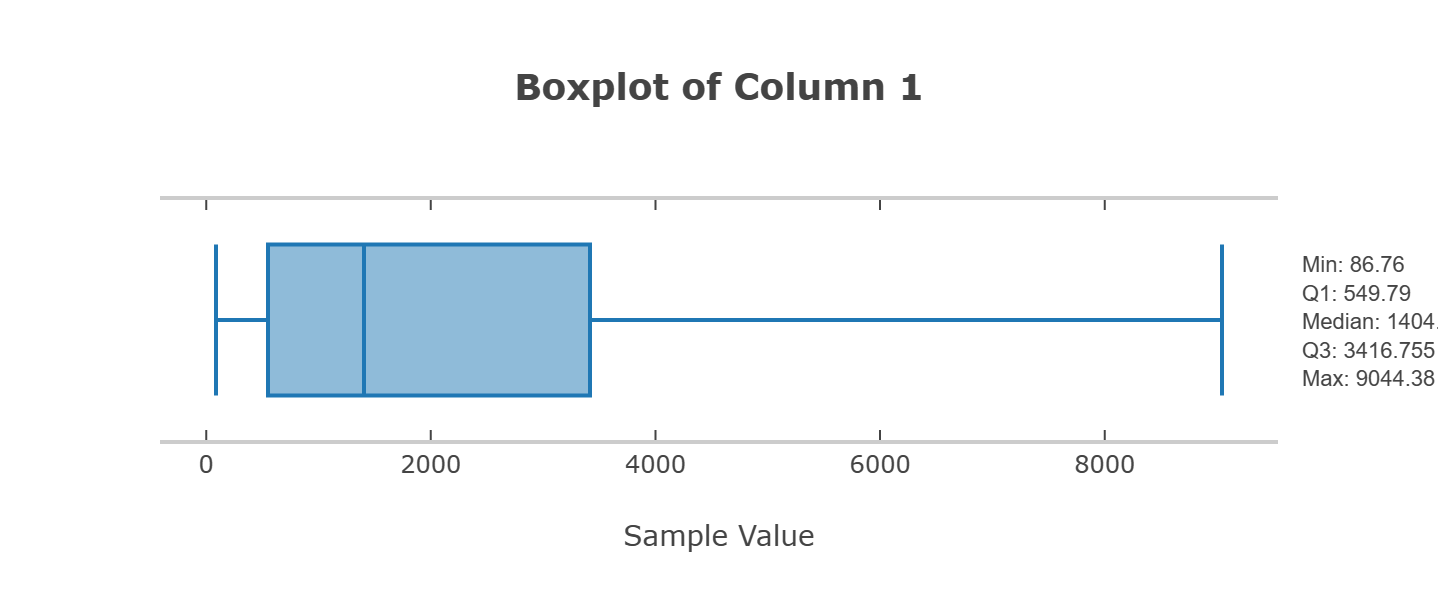
\includegraphics[width=0.8\linewidth]{statdisk_boxplot_q8.png}
              \caption{Boxplot}
              \label{fig:boxplot_q8}
          \end{figure}

          \begin{figure}[H]
              \centering
              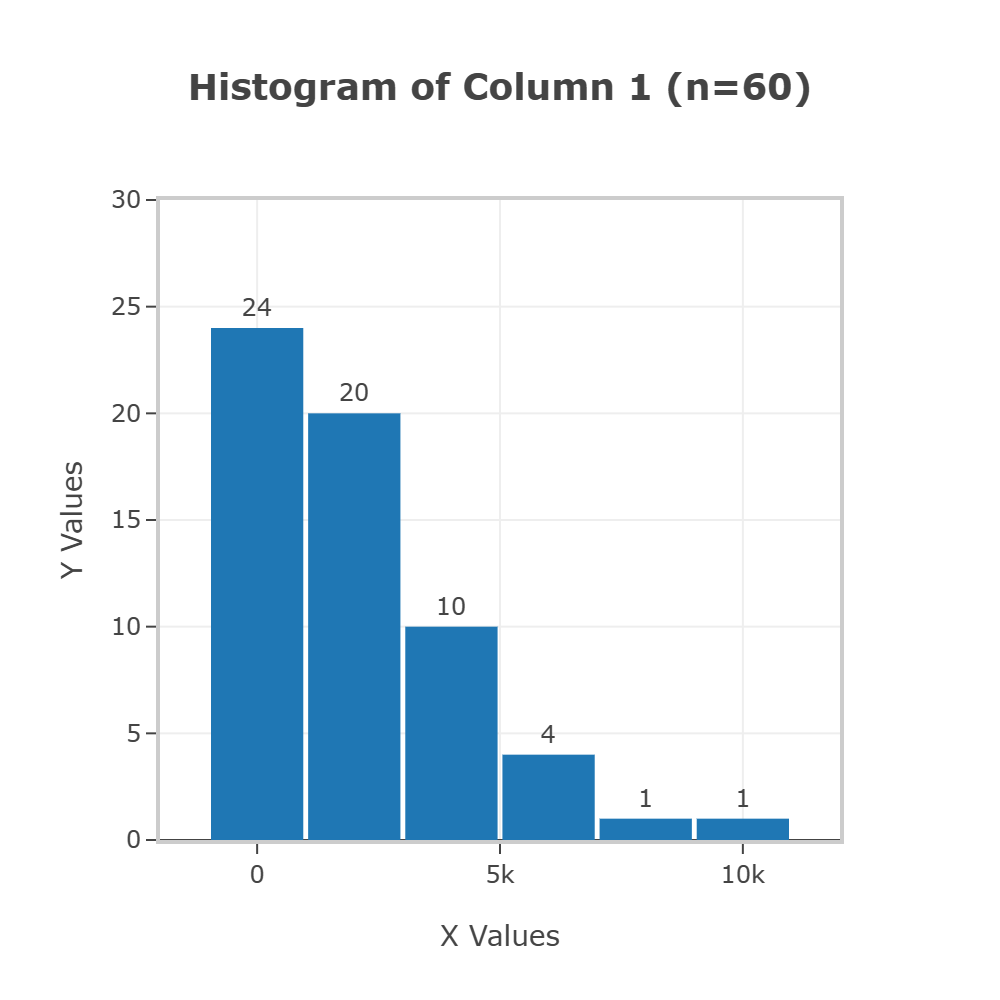
\includegraphics[width=0.8\linewidth]{statdisk_histogram_q8.png}
              \caption{Histogram}
              \label{fig:histogram_q8}
          \end{figure}

          \begin{figure}[H]
              \centering
              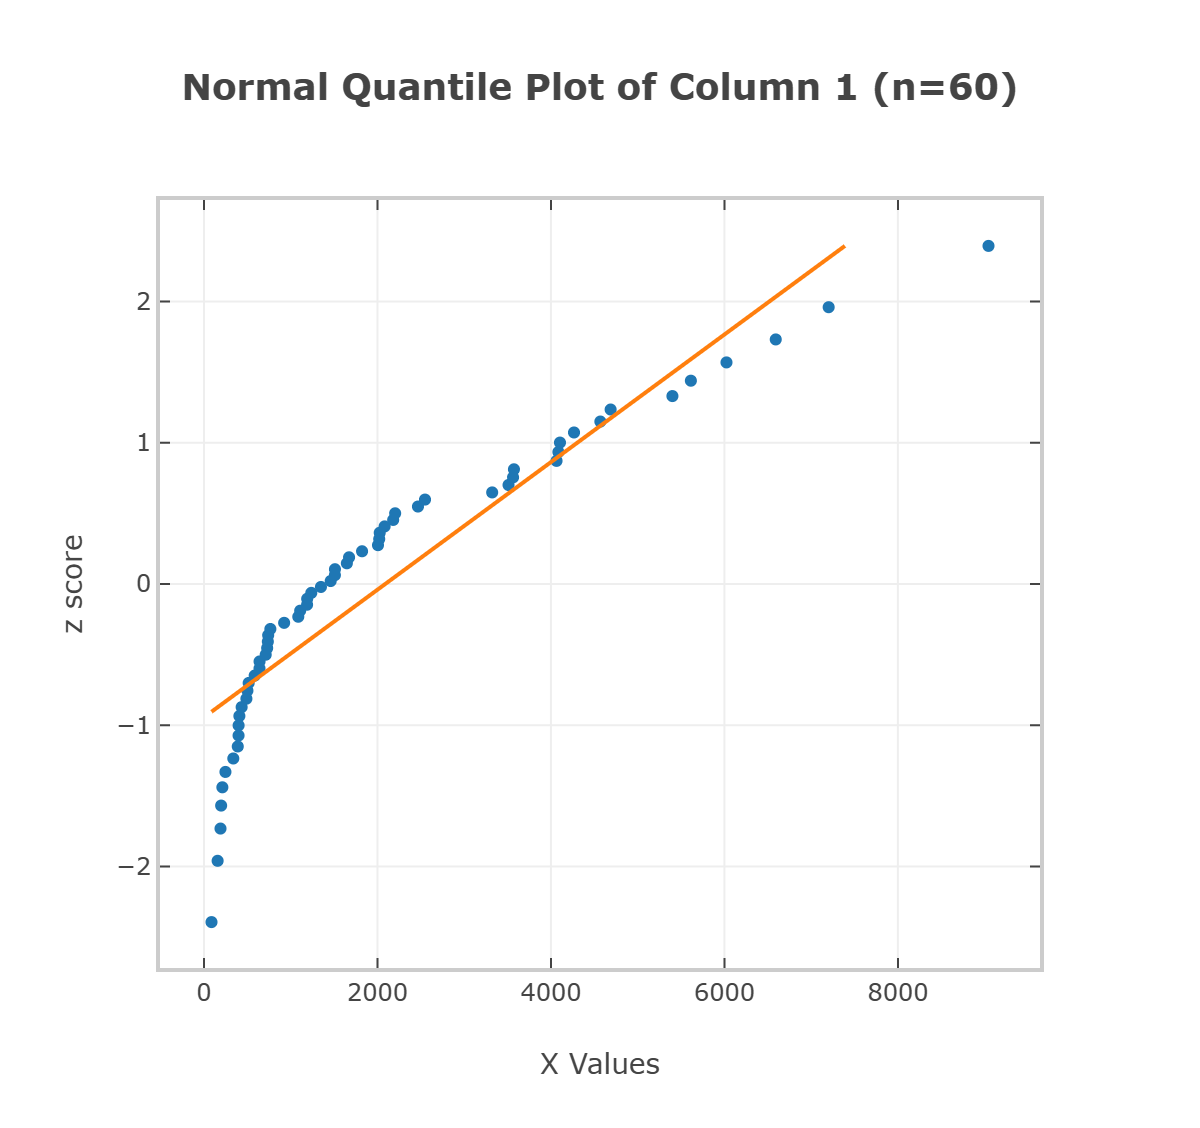
\includegraphics[width=0.8\linewidth]{statdisk_normal_quantile_plot_q8.png}
              \caption{Normal Quantile Plot}
              \label{fig:normalquantile_q8}
          \end{figure}

          According to \ref{fig:normalquantile_q8} we can already discard the Normal distribution. Based on the Box Plot in \ref{fig:boxplot_q8} and the Histogram in \ref{fig:histogram_q8} a good guess would be the exponential distribution.

    \item Before conducting the the goodness of fitting it is necessary to estimate the distribution parameter $\lambda$ for $f(t)=\lambda e^{-\lambda t}$, to do it, it can be used the maximum likelihood method, it can be done substituting the obtained values for the distribution on the following equation:

          \begin{equation}
              \lambda=\frac{n}{\sum\limits_{i=1}^{n}t_i}
          \end{equation}


          where $n=60$ and $\sum\limits_{i=1}^{n}t_i=125378.40$. so the value for $\lambda$ is:
          \begin{empheq}[box=\fbox]{align*}
              \lambda\approx 0.0004786
          \end{empheq}

          The Kolmogorov Smirnov can be used to check if the distribution fits:
          \begin{figure}[H]
              \centering
              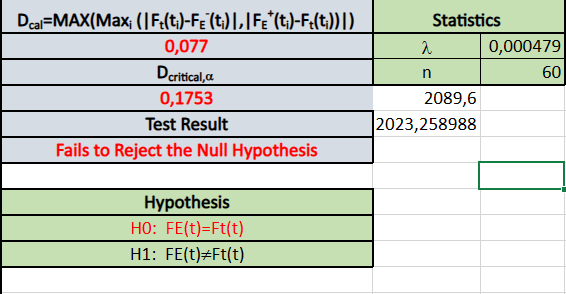
\includegraphics[width=0.7\linewidth]{ks_q8.png}
              \caption{Kolmogorov Smirnov Method}
              \label{fig:graphical2_q8}
          \end{figure}

          As the Kolmogorov Smirnov test failed to reject the null hypothesis so it is safe to assume
          the exponential distribution may fit the data.

          \begin{figure}[H]
              \centering
              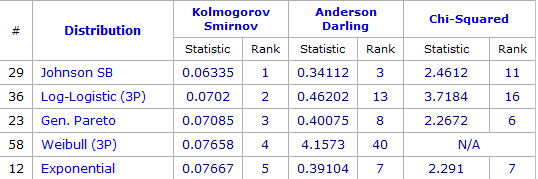
\includegraphics[width=0.7\linewidth]{easyfit_q8.png}
              \caption{Easy Fit}
              \label{fig:easyfit_q8}
          \end{figure}

          Using easy fit to check if the exponential method it can be seem that the exponential distribution ranks pretty high among the possible distributions that can fit the data using the Kolmogrov Smirnov, Anderson Darling and Chi-Squared methods, There are better distributions according to Easy Fit for the data, but it will be used the exponential distribution because it was the one first assumed and the null hypothesis was not rejected.

    \item An estimation for $MTTF$ can be obtained by simply taking the mean from the failure time on the table, or by calculating $1/\lambda$. The result obtained after doing this is:

          \begin{empheq}[box=\fbox]{align*}
              MTTF = \frac{\sum\limits_{i=1}^{n}t_i}{n} = 2089.64
          \end{empheq}


    \item Using the following code in python to apply the semi-parametric bootstrap to the data:

          \lstset{
              basicstyle=\ttfamily,
              numbers=left,
              numberstyle=\tiny\color{gray},
              breaklines=true,
              keywordstyle=\color{blue},
              commentstyle=\color{green!40!black},
              stringstyle=\color{orange},
              frame=single,
              language=Python
          }


          \begin{lstlisting}
    import numpy as np
    
    data = [765.32, 1822.54, 515.21, 4569.68, 408.16, 338.18, 736.36, 2026.03, 5400.53, 4104.01, 1509.31, 197.89, 4688.02, 211.91, 1460.71, 728.45, 434.26, 584.37, 2181.27, 1109.13, 1672.6, 1188.55, 2005.96, 86.76, 4085.9, 1189.89, 640.21, 640.83, 924.12, 2204.17, 9044.38, 1348.37, 711.69, 5613.1, 1510.17, 6591.52, 3573.45, 389.56, 190.62, 247.44, 2548.0, 6023.71, 7201.78, 3563.3, 4266.0, 1647.28, 157.32, 398.62, 1237.32, 2082.53, 1087.26, 500.76, 399.17, 4064.59, 740.13, 3322.64, 489.08, 3510.87, 2020.38, 2467.03]
    data.sort()
    data = np.array(data)
    iterations = 1000
    MTTF = np.mean(data)
    mttfs = []
    
    for _ in range(iterations):
      # non_parametric_data = np.random.choice(data,size=len(data),replace=True)
      parametric_data = np.random.exponential(scale=MTTF, size=len(data))
      mttfs.append(np.mean(parametric_data))
    
    mttfs.sort()
    confidence_interval = np.percentile(mttfs, [2.5, 97.5])
    print(confidence_interval)
    \end{lstlisting}

          the confidence interval for $MTTF$ with 5\% of significance is :


          \begin{empheq}[box=\fbox]{align*}
              [1624.6652h,~2631.3845h]
          \end{empheq}

    \item
    For an exponential distribution the Reliability function is:
    \begin{equation}
        R(t)=e^{-\lambda t}=e{-0.0004786 t}
    \end{equation}

    so for $t=1000h$ then:
    \begin{empheq}[box=\fbox]{align*}
        R(t=1000)=e^{-0.0004786 \cdot 1000} \approx 0.619
    \end{empheq}

    For an exponential distribution the Failure function is:
    \begin{equation}
        F(t)=1-R(t)
    \end{equation}

    so for $t=1000h$ then:
    \begin{empheq}[box=\fbox]{align*}
        F(t=1000)=1-0.619 \approx 0.380
    \end{empheq}

    For an exponential distribution the density function is:
    \begin{equation}
        f(t)=\lambda e^{-\lambda t}=0.0004786\cdot e^{-0.0004786 t}
    \end{equation}

    So for $t=1000h$ then:
    \begin{empheq}[box=\fbox]{align*}
        f(t=1000)=0.0004786\cdot e^{-0.0004786 \cdot 1000} \approx 0.000297
    \end{empheq}
    For an exponential distribution the hazard function is constant:

    \begin{equation}
        \lambda(t)=\lambda=0.0004786
    \end{equation}

    So for $t=1000h$ then:
    \begin{empheq}[box=\fbox]{align*}
        \lambda(t=1000)=\lambda=0.0004786
    \end{empheq}
\end{enumerate}

%----------------------------------------------------------------------------------------
%	PROBLEM 9
%----------------------------------------------------------------------------------------
\setcounter{Question}{8}
\begin{question}
    Consider the reliability experiment in which sixty servers \((n = 60)\) were observed in an accelerated reliability test. The times each server failed were recorded in Table 4 (complete data). Using a non-parametric method, calculate
    \begin{enumerate}[label=(\alph*)]
        \item \(\hat{R}(t) \text{ at } t = 1000h\)
        \item \(\hat{F}(t) \text{ at } t = 1000h\)
        \item \(\hat{f}(t) \text{ at } t = 1000h\)
        \item \(\hat{\lambda}(t) \text{ at } t = 1000h\)
    \end{enumerate}
    Draw:
    \begin{enumerate}[label=(\alph*), start=5]
        \item \(\hat{R}(t_i) \times t_i\)
        \item \(\hat{F}(t_i) \times t_i\)
        \item \(\hat{f}(t_i) \times t_i\)
        \item \(\hat{\lambda}(t) \times t\)
    \end{enumerate}
    And:
    \begin{enumerate}[label=(\alph*), start=9]
        \item \(\widehat{MTTF}\)
        \item Estimate the confidence interval using non-parametric bootstrap.
        \item Compare the results with Exercise 8 and comment.
    \end{enumerate}
\end{question}

As we have ungrouped and complete reliability data, we can use a simple method to estimate each function. All the data was gathered in an Excel sheet, and the following equations were used for non-parametrically estimating the desired functions:
    \begin{align*}
        \hat{R}(t_i) &= \frac{n+1-i}{n+1}    &   \hat{F}(t_i) &= \frac{i}{n+1} \\
        \hat{f}(t_i) &= \frac{1}{(n+1)(t_i - t_{i - 1})}   &   \hat{\lambda}(t_i) &= \frac{1}{(n+1-i)(t_i - t_{i-1})}
    \end{align*}
    Where $(n - i)$ is the number of surviving servers at time $t_i$. Some of the calculated results can be seen in the following table:

    \begin{table}[H]
        \centering
        \caption{Estimated functions}
        \label{tab:my-table}
        \begin{tabular}{|c|c|cccc|}
            \hline
            $i$ & $t_i$ & $R(t_i)$ & $F(t_i)$ & $f(t_i)$ & $l(t_i)$ \\
            \hline
            1  & 86.76  & 0.9836 & 0.0164 & 0.0000 & 0.0000 \\
            2  & 157.32 & 0.9672 & 0.0328 & 0.0002 & 0.0002 \\
            3  & 190.62 & 0.9508 & 0.0492 & 0.0005 & 0.0005 \\
            4  & 197.89 & 0.9344 & 0.0656 & 0.0023 & 0.0024 \\
            5  & 211.91 & 0.9180 & 0.0820 & 0.0012 & 0.0013 \\
            $\cdots$ & $\cdots$ & $\cdots$ & $\cdots$ & $\cdots$ & $\cdots$ \\
            20 & 728.45 & 0.6721 & 0.3279 & 0.0010 & 0.0015 \\
            21 & 736.36 & 0.6557 & 0.3443 & 0.0021 & 0.0032 \\
            22 & 740.13 & 0.6393 & 0.3607 & 0.0043 & 0.0068 \\
            23 & 765.32 & 0.6230 & 0.3770 & 0.0007 & 0.0010 \\
            24 & 924.12 & 0.6066 & 0.3934 & 0.0001 & 0.0002 \\
            25 & 1087.26 & 0.5902 & 0.4098 & 0.0001 & 0.0002 \\
            26 & 1109.13 & 0.5738 & 0.4262 & 0.0007 & 0.0013 \\
            27 & 1188.55 & 0.5574 & 0.4426 & 0.0002 & 0.0004 \\
            28 & 1189.89 & 0.5410 & 0.4590 & 0.0122 & 0.0226 \\
            $\cdots$ & $\cdots$ & $\cdots$ & $\cdots$ & $\cdots$ & $\cdots$ \\
            55 & 5400.53 & 0.0984 & 0.9016 & 0.0000 & 0.0002 \\
            56 & 5613.1 & 0.0820 & 0.9180 & 0.0001 & 0.0009 \\
            57 & 6023.71 & 0.0656 & 0.9344 & 0.0000 & 0.0006 \\
            58 & 6591.52 & 0.0492 & 0.9508 & 0.0000 & 0.0006 \\
            59 & 7201.78 & 0.0328 & 0.9672 & 0.0000 & 0.0008 \\
            60 & 9044.38 & 0.0164 & 0.9836 & 0.0000 & 0.0005 \\
            \hline
        \end{tabular}
    \end{table}

    With the calculated data, we can then use the following formula to calculate the values for each function at $t = 1000$:
    \[\hat{R} = (t_j) = a \times t_j + b\]
    Where $t_i < t_j < t_{i+1}$, such that $t_j$ is the desired $t$, and $t_i, t_{i+1}$ are two recorded failure times, and
    \[a = \frac{\hat{R}(t_{i+1})- \hat{R}(t_i)}{t_{i+1} - t_i}\]
    \[b = \hat{R}(t_i) - a \times t_i\]

    \begin{enumerate}[label=(\alph*)]
        \item We choose $i = 24$ for our estimation, as $924.12 < 1000 < 1087.26$. Therefore, we have:
        \begin{gather*}
            a = \frac{0.5902 - 0.6066}{1087.26 - 924.12} = \num{-1,0052e-4} \\
            b = 0.6066 - (\num{-1,0052e-4} \times 924.12) = 0,6994 \\
            \hat{R}(1000) = (\num{-1,0052e-4} \times 1000) + 0,6994 \\
            \fbox{$\hat{R}(1000) = 0,5988$}
        \end{gather*}
        \item Using a similar approach, we can calculate the rest of the functions at $t = 1000$
        \[\fbox{$\hat{F}(1000) = 0.4010$}\]
        \item \[\fbox{$\hat{f}(1000) = 0.0001$}\]
        \item \[\fbox{$\hat{\lambda}(1000) = 0.0001$}\]
        \item $R(t)$
        \begin{figure}[H]
            \centering
            \includegraphics[width=0.8\linewidth]{q9_rt.png}
            \caption{$\hat{R}(t) \times t$}
            \label{fig:q9_rt}
        \end{figure}
        \item $F(t)$
        \begin{figure}[H]
            \centering
            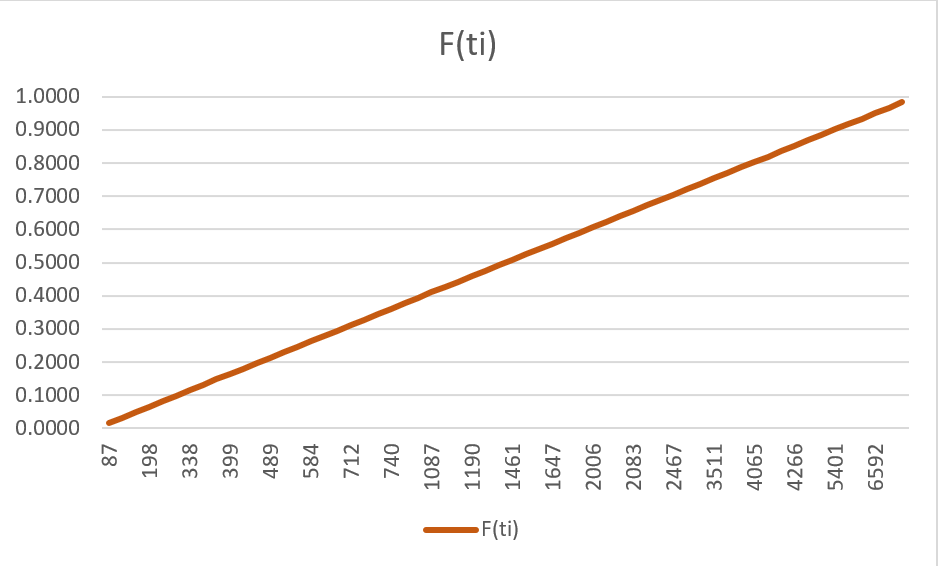
\includegraphics[width=0.8\linewidth]{q9_FFt.png}
            \caption{$\hat{F}(t) \times t$}
            \label{fig:q9_Ft}
        \end{figure}
        \item $f(t)$
        \begin{figure}[H]
            \centering
            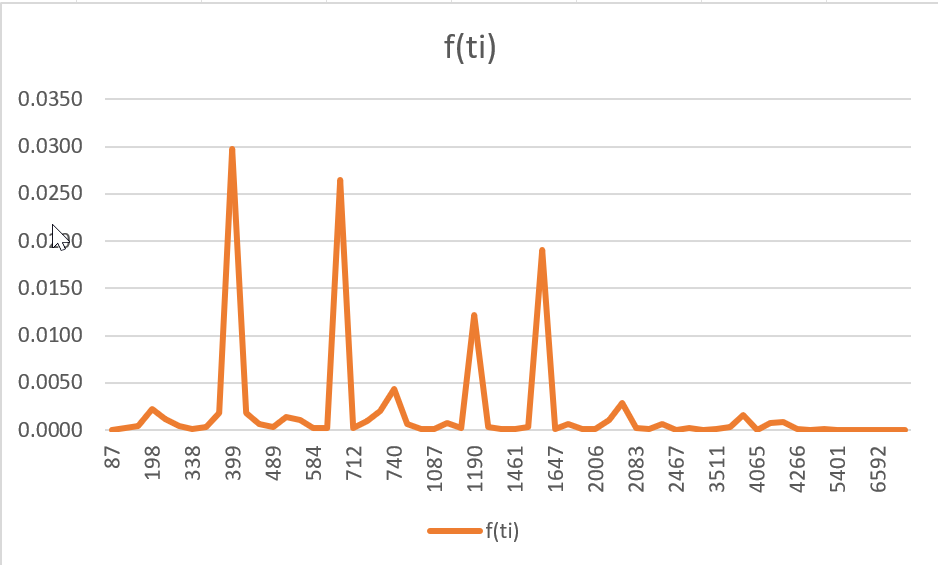
\includegraphics[width=0.8\linewidth]{q9_ft.png}
            \caption{$\hat{F}(t) \times t$}
            \label{fig:q9_ft}
        \end{figure}
        \item $\lambda(t)$
        \begin{figure}[H]
            \centering
            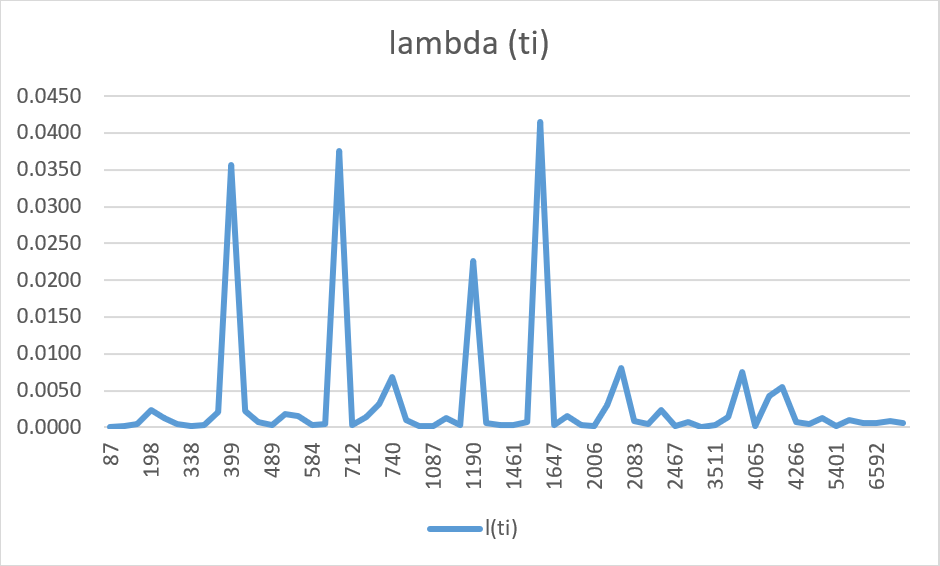
\includegraphics[width=0.8\linewidth]{q9Lt.png}
            \caption{$\hat{F}(t) \times t$}
            \label{fig:q9_lt}
        \end{figure}
        \item The MTTF is estimated by
        \[\widehat{MTTF} = \frac{\sum_{i=1}^{n}t_i}{n}\]
        Computing this, we get:
        \[\fbox{$MTTF = 2089.64h$}\]
        \item Assuming a confidence level of 95\%, upon calculating the confidence interval using non-parametric bootstrap, we get \fbox{MTTF $\in (1599.03h,~ 2609.37h)$}
        \item The results compared to the ones found in Exercise 8 are very close, which demonstrates that the semi-parametric approach chosen in the previous exercise seems to accurately represent the original dataset.
    \end{enumerate}
    
\end{document}
